\chapter{Design}


\section{Project Contribution}
\label{contribution}

We thus arrive at the intended innovation behind the project idea - to create a semi-automated web application vulnerability scanner. The essential difference between this and the aforementioned black box scanners is that it intends to work as an aide alongside a pentester, not as a fully automated background process, leveraging its role as a Chrome Extension. \\

The proposition of creating a tool that is driven by user input seems appealing for a number of reasons:

\begin{itemize}
	\item \textbf{Full Experience} - A scanner that analyses a web application for vulnerabilities as a user is using the application has fewer limitations as to what is within its scope. As pointed out by \cite{whyJohnnyCantPentest}, scanners struggle to scour through more complex constructs of the internet such as convoluted Javascript forms, AJAX requests and Flash objects. As a result, many scanners ignore these features altogether, dismissing potential vulnerabilities in the process. A user driven experience allows the user to interact as they would normally with these technologies, and can analyse inputs and outputs accordingly.
	
	\item \textbf{Educational} - As mentioned in the introduction, one of the issues that leads to the need of vulnerability scanners is the lack of security-aware developers. By developing a tool that works alongside developers, they can refine their skills in this area if they already know some security basics. There is also room for learning for website owners as penetration testers may demonstrate the severity of exploits caused by vulnerabilities using the tool, and mitigating these. 
	
	\item \textbf{Simpler crawling module} - Since the tool is not scouring the entire site at once but is rather following the more natural workflow of a human user, the equivalent crawling module will only need to keep a much smaller representation of the website as opposed to before. A proposed methodology to simplify this process given the project specification is to create a crawler based on recommendations and an 'action replay' mechanism. 
	
	The recommendation algorithm will need to be based off of similar existing algorithms in automatic crawlers. Since the tool must be driven by user input, the crawler would analyse contents and interactions of the web application with the user (as it would do automatically), and suggest specific features to the user as a starting point for the scan. This can be done by passively reading the contents of web requests between the user and the web application and flagging up any that seem to exhibit behaviour of an insecure system, such as passing user inputs in clear text, or using client-side inputs to control important application sensitive logic. Once a user chooses to follow a recommendation, they may investigate the flagged feature more closely.
	
	At this point, the 'action replay' algorithm begins - once a user has elected a potential target to test for a vulnerability, the tool begins to record user actions. Depending on the selected feature and what vulnerabilities may be discoverable, the tool can then suggest a stopping point of recording, or wait for the user to determine when their actions that detect a vulnerability are enough. The tool then takes these actions and analyses their outputs - it may be the case that a user has found a vulnerability on their first go. It could also be the case that this input didn't trigger a vulnerability, but is worth looking into further. At this point, the crawler will begin to fuzz different versions of input that may be more effective at showcasing vulnerabilities. In recent research by Parvez et al. into evaluating black box scanners \cite{analysisOfEffectivenessOfBlackBoxWebAppScannersStoredSQLStoredXSS}, one of the final recommendations for a better scanner was to add interactive multistep options to the scanner, which is a main focus of this method. To the best of my knowledge, this 'action replay' algorithm is a novel approach in this area.
	
	\begin{figure}[h]
		\centering
		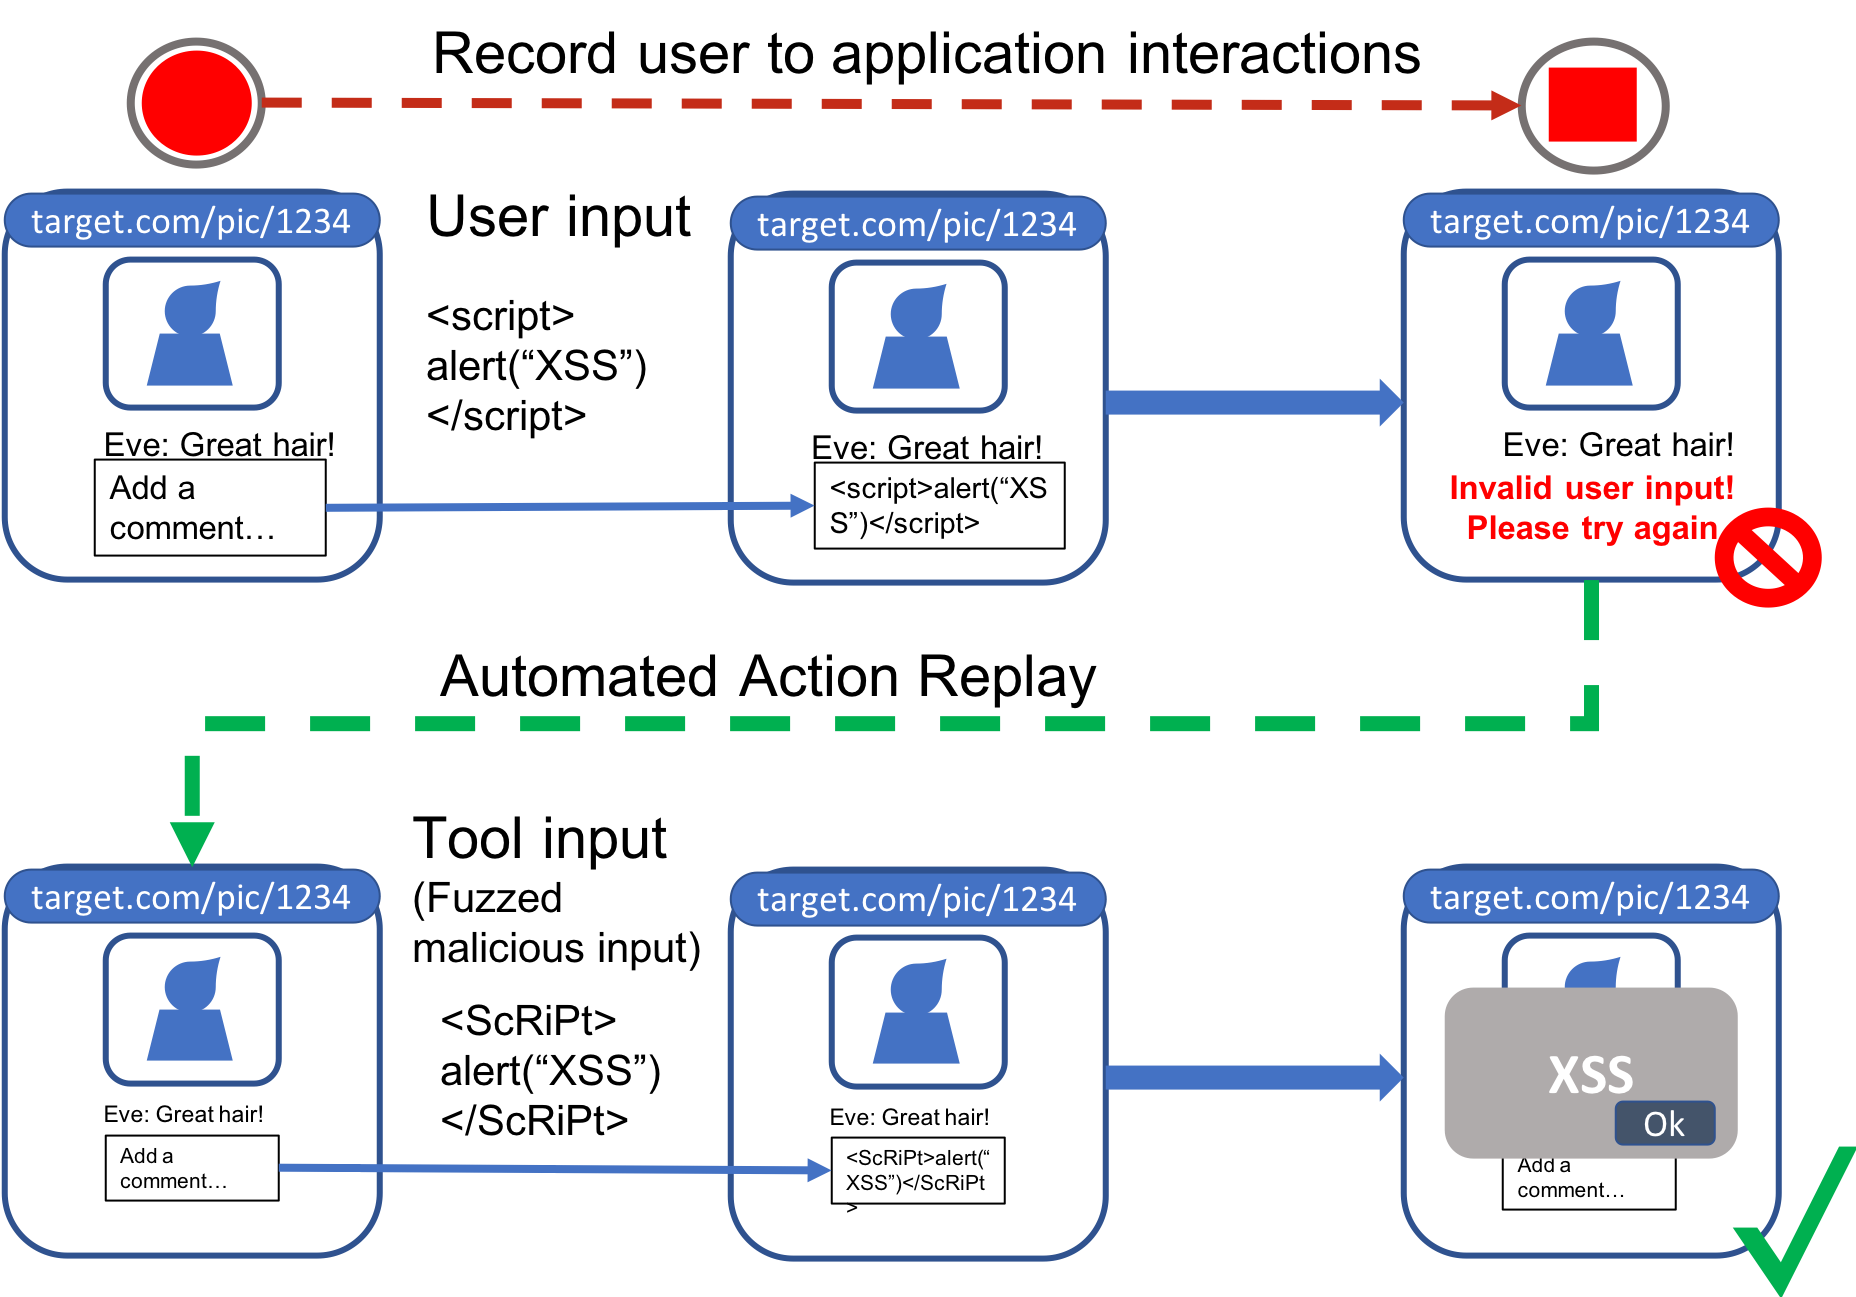
\includegraphics[width=\textwidth]{images/action_replay.png}
		\caption{A visualization of the proposed action replay algorithm. The tool records user input for a time period determined by the user. The tool then replicates actions using fuzzed inputs to try and uncover vulnerabilities if the first attempt was unsuccessful.}
		\label{fig:test}
	\end{figure}
	
	
	\item \textbf{Human judgement} - The previously mentioned paper by Parvez et al. also mentions that choosing the right attack vectors to exploit vulnerabilities is still a big challenge for black box scanners \cite{analysisOfEffectivenessOfBlackBoxWebAppScannersStoredSQLStoredXSS}. Huang et al. recently built a scanner that performed well against open-source competition \cite{webAppSecThreatsCountermeasuresPitfalls}. However, these authors recently acknowledge that \emph{"there is no silver bullet for web application security; threats will continue to grow and evolve"}. Herein lies much of the motivation for making this project user-centric: vulnerability detection and even exploitation may be automated \cite{darpaAIChallenge}, but for now, efforts in having to build an AI that is able to do this are astronomical - it takes years for teams of experts to build tools that do this. Following its recent success, the winner of the DARPA Cyber Grand Challenge (an AI-only capture the flag contest) was pitted against human professionals at the 2016 DEF CON CTF Challenge, where it came last \cite{defcon16Results}. These efforts show a bright future for fully automated security systems, but these may still be some years away in the full making. This project does not admit defeat in attempting to automate the process of countering malicious agents, but rather aims to increase the likelihood of doing a good job against them by covering our bases with higher quality base defences. In fact, even limited domain knowledge has shown to be useful for human penetration testers; a group of students with 'average' security skills achieved a higher success rate on their own than some vulnerability scanners in analysing web applications \cite{whyJohnnyCantPentest}. It is hoped that with the correct suggestions provided by the tool, this project lowers the minimum requirements of a successful user to be 'below average' in their security domain knowledge. \\
	
\end{itemize}



\section{Limitations}
\label{limitations}

In order to be able to effectively evaluate this project at a later point, it is important to delineate realistic expectations in terms of what it can and cannot do. 

\subsection{Time taken}
Since the extension is user driven and not fully automatic, the suggested process will be inevitably slower than if it was otherwise automated - there will be waiting times as users will not instantly attempt to uncover recommended vulnerabilities. There may also be some intellectual effort involved in crafting initial input to try and do this, which adds to this. Both of these factors add to 2 different metrics: the total scan time and the time taken from recommendation to decision of whether a vulnerability is found or not. \\

Total scan time may be especially hard to measure, and can be seen as a disadvantage of this scan. It is not known whether a user will eventually go through every possible page that is relevant, so it becomes very difficult to claim an end to the scan. On the contrary, automated crawlers \emph{will eventually} come to an end their search, and thus put an upper bound on how many resources they can analyse. Human driven crawling may stop or resume at any given point. Not being able to best assess the total scan time is an acceptable tradeoff of this project as it will simply not be avoidable given human driven interaction is being explored. \\

The time taken to ascertain whether a vulnerability exists or not from a recommendation can however be bounded. This period begins when a user decides to investigate a recommendation on their own or by suggestion of the tool, and finishes either when enough proof of a vulnerability has been observed, or when all possible fuzzing opportunities in exploiting it have been exhausted - the extension will have a list of possible fuzzing mutations per type of vulnerability, so this work is bounded by that list. Again, since this is not a fully automated tool, the extension is expected to take longer in this metric due to human interaction when comparing it to automated scanners, which is only natural. \\

\subsection{Breadth of  work}
Section \ref{vulnerabilities} describes many potential kinds of vulnerabilities that the project may choose to tackle. Some of these are harder to detect than others, and thus require more development work. This large scope may make it tempting to try and undertake too many things at once. At the time of writing, it is also hard to assess just how difficult it may be to implement scanning for a specific type of vulnerability. The extension will be developed with aims of finding revelant vulnerabilities - sorted by both volume of occurrence and contemporary relevance as found on surveys. One of the most recurring vulnerabilities in both aspects is Cross Site Scripting, so developing the tool to be able to detect this class of weaknesses is a good starting point. Other features that may seem small (such as analysing cookies or the use of iFrames on a page), may also be beneficial to implement. As the project develops, it becomes harder to weigh the costs of effort to implement versus the success rate of focusing on a specific feature, so some further time should be allocated to allow for this meta research. \\ 

\subsection{Self security}
The security of the extension being developed should not be taken for granted. As mentioned above, Google Chrome has several mechanisms in place to safeguard extensions from falling prey to malicious attackers. Namely, these are:
\begin{itemize}
	\item \textit{Isolated Worlds}
	\item Privilege separation
	\item Predefined permissions
	\item CSP (Content Security Policy)
\end{itemize} 
Although these practices make it much easier for a developer to avoid serious mistakes, it is still possible to write vulnerable extensions. The \textit{threat model} in this case (the way we choose to archetype our potential enemy), is by means of a web attacker. This would be someone who sets up a 'honeypot' website, expecting the extension to scan it but in the process attempt to compromise the extension by different means. Due to the priveleges granted to an extension, this may result in the jeopardizing of sensitive user data, such as their passwords. A recent paper by Carlini, Felt and Wagner reinforces the notion that Chrome's existing techniques are effective in preventing extension compromise, but also list some developer practices that could result in vulnerabilities, such as the unrestricted use of the \texttt{eval} function by Javascript (which is known to be dangerous as it executes given strings as commands), and injecting website data into HTML \cite{evalChromeExtensionSecurityArchitecture}. Many of the notions mentioned in the paper are also cited in Google's own documentation on how to write Chrome extensions \cite{chromeExtensionArchitecture}. Following these best practices will decrease potential risks associated with this project. \\ 

\subsection{Ethics \& Handling of Results}
\label{ethics}
This project aims to build a tool that helps users find vulnerabilities in web applications. Obviously, this may raise ethical ramifications as to how the tool interacts with websites, and how its output is handled. \\

As the tool needs to send requests on the user behalf when executing (especially so during the 'action replay' phase described above), the rate at which this is done may be of concern. Conventional automated scanners may fire 100's of different fuzz attempts at a web application, \emph{per vulnerability, per existing page} - a shotgun-like approach. This approach is very intensive, and for web applications set up for smaller amounts of traffic, may result in a Denial of Service (DoS). This tool aims to reduce this by only passively reading user crawled content, and only actively interacting with the website whenever a flagged vulnerability has been detected. \\

A related concern is to do with the scope of testing and uses on a real web application. For testing and evaluation purposes, the tool will be ran against existing, known to be vulnerable applications, such as DVWA \cite{dvwaSite}. Ideally, it should also be ran against other web applications beyond my control. However, for some of these, it may be the case that running the unhinged extension may infringe usage terms and agreements. For this purpose, a proposed restrained mode for the tool may be built, such that it does not actively take any action when browsing web applications, but rather only passively reads network traffic to deduce and recommend potential vulnerabilities. \\

Naturally, as per the project ideals, any vulnerabilities that may be found as a result of running this extension will duly be reported to the appropriate developers.